\documentclass[12pt, a4paper]{article}

% Set relative path to all figures
\newcommand*{\floatRelativePathTwentyFive}{../out/gwas417/pval_5e-08/r2_0.1/kb_1000/window_1000000/75_25}%
\newcommand*{\floatRelativePath}{../out/gwas417/pval_5e-08/r2_0.1/kb_1000/window_1000000/75_50}%
\newcommand*{\floatRelativePathSeventyFive}{../out/gwas417/pval_5e-08/r2_0.1/kb_1000/window_1000000/75_75}%

\usepackage[utf8]{inputenc}
\usepackage{csvsimple}
\usepackage{graphicx}
\usepackage{hyperref}
\usepackage{nameref}
% \usepackage{natbib}
\usepackage{subcaption}
\usepackage{biblatex}
\addbibresource{/home/gonzalez/Repositories/gwas2eqtl_pleiotropy/ms/ms_pleiotropy.bib}
% \addbibresource{\jobname.bib}

%\captionsetup[figure]{labelfont={bf},labelformat={default},labelsep=period,name={Fig.}}

\begin{document}

%%%%%%%%%%%%%%%%%%%%%%%%%%%%%%%%%%%%%%%%%%%%%%%%%%%%%%%%%%%%%%%%%%%%%%%%%%%%%%%%
%
% Tab 1: Representative pleiotropic eQTLs of cytobands
%
%%%%%%%%%%%%%%%%%%%%%%%%%%%%%%%%%%%%%%%%%%%%%%%%%%%%%%%%%%%%%%%%%%%%%%%%%%%%%%%%

\begin{table}[!ht]
    \centering
    \scriptsize

    \csvreader[separator=tab,
    tabular=crclcp{0.4\textwidth},
    late after last line=\\\hline,
    head,
    table head=\\\hline \bfseries Chrom. & \bfseries Pos (hg38) & \bfseries Cytoband & \bfseries RSID & \bfseries Gene marker& \bfseries Trait categories\\\hline,
    ]{\floatRelativePath/cmpt_count_per_rsid.py/count_per_rsid_gwas_ms.tsv}{}% use head of csv as column names
        {\csvcoli\ & \csvcolii\ & \csvcoliii\ & \csvcoliv\ & \csvcolv\ & \csvcolvi}% specify your coloumns here
    %
    \vspace{15pt}
    %
    \caption{
%        Represantive pleiotropic eQTLs involved in four GWAS categories in different cytobands.
%    The gene marker is the eQTL gene with the highest PubMed publication count.
%    The whole list is given in the Supplementary table ST2.
    }
    \label{tab:pleitropic_eqtls}
\end{table}

%%%%%%%%%%%%%%%%%%%%%%%%%%%%%%%%%%%%%%%%%%%%%%%%%%%%%%%%%%%%%%%%%%%%%%%%%%%%%%%%
%
% Tab 2: Region containing most pleiotropic eQTLs
%
%%%%%%%%%%%%%%%%%%%%%%%%%%%%%%%%%%%%%%%%%%%%%%%%%%%%%%%%%%%%%%%%%%%%%%%%%%%%%%%%

\begin{table}[!ht]
    \centering
    \scriptsize
    \csvreader[
        separator=tab,
        tabular=p{0.03\textwidth}p{0.1\textwidth}p{0.1\textwidth}p{0.06\textwidth}p{0.08\textwidth}p{0.45\textwidth}p{0.08\textwidth}p{0.08\textwidth},
        late after last line=\\\hline,
        head,
        table head=\\\hline \bfseries Chr. & \bfseries Start & \bfseries End & \bfseries Cytob. & \bfseries Marker eQTL gene & \bfseries Trait categories & \bfseries Length & \bfseries eQTLs cnt.\\\hline,
    ]{\floatRelativePath/cmpt_pleiotropic_regions.py/100000/region_window_ms.tsv}{}% use head of csv as column names
    {\csvcoli\ & \csvcolii\ & \csvcoliii\ & \csvcoliv\ & \csvcolv\ & \csvcolvi\ & \csvcolvii\ & \csvcolviii}% specify your coloumns here
    %
    \vspace{15pt}
    %
    \caption{
%        Pleiotropic regions involving 6 or more GWAS classes. These regions were built with a sliding window of 1e5 nt. Genomic coordinates are given for the hg38 assembly.
    }\label{tab:pleiotropic_regions}
    %
\end{table}

%%%%%%%%%%%%%%%%%%%%%%%%%%%%%%%%%%%%%%%%%%%%%%%%%%%%%%%%%%%%%%%%%%%%%%%%%%%%%%%%
%
% Fig 1a-d: Histogram of percentage of explained of GWAS
% Fig 1e: Trait distance matrix
%
%%%%%%%%%%%%%%%%%%%%%%%%%%%%%%%%%%%%%%%%%%%%%%%%%%%%%%%%%%%%%%%%%%%%%%%%%%%%%%%%

\begin{figure}[!tbp]
    \centering

    \begin{subfigure}[]{0.65\textwidth}
        \textbf{a}
        \\
        \includegraphics[width=\textwidth]{\floatRelativePath/cmpt_perc_tophits_eqtl.py/loci_explained_perc.png}
    \end{subfigure}

    \begin{subfigure}[]{0.85\textwidth}
        \textbf{b}
        \\
        \includegraphics[width=\textwidth]{\floatRelativePath/plthtmp_disease_comorbidity_matrix.py/corr_inkscape.png}
    \end{subfigure}

    \caption{}
%
\end{figure}

%%%%%%%%%%%%%%%%%%%%%%%%%%%%%%%%%%%%%%%%%%%%%%%%%%%%%%%%%%%%%%%%%%%%%%%%%%%%%%%%
%
% Fig 2: Length histogram of regions
% Fig 3: Histograms of variants vs GWAS, eQTL genes and eQTL biosamples
% Fig: Spearman correlation between counts of GWAS categories, eQTL genes and eQTL biosamples
% Fig: VEP consequences
%
%%%%%%%%%%%%%%%%%%%%%%%%%%%%%%%%%%%%%%%%%%%%%%%%%%%%%%%%%%%%%%%%%%%%%%%%%%%%%%%%

\begin{figure}[!ht]
    %
    \centering

    \begin{subfigure}[]{.49\textwidth}
        \textbf{a}
        \\
        \includegraphics[width=\textwidth]{\floatRelativePath/plthst_gwas_egene_etissue.py/hist_gwas.png}
    \end{subfigure}
    %
    \begin{subfigure}[]{.49\textwidth}
        \textbf{b}
        \\
        \includegraphics[width=\textwidth]{\floatRelativePath/plthst_gwas_egene_etissue.py/hist_egene.png}
    \end{subfigure}

    \begin{subfigure}[]{.49\textwidth}
        \textbf{c}
        \\
        \includegraphics[width=\textwidth]{\floatRelativePath/plthst_gwas_egene_etissue.py/hist_etissue.png}
    \end{subfigure}
    %
    \begin{subfigure}[]{.49\textwidth}
        \textbf{d}
        \\
        \includegraphics[width=\textwidth]{\floatRelativePath/cmpt_count_per_rsid.py/count_per_rsid_gwas_egene_etissue_corr.png}
    \end{subfigure}

    \begin{subfigure}[]{.49\textwidth}
        \textbf{e}
        \\
        \includegraphics[width=\textwidth]{\floatRelativePath/pltbar_pleiotropic_regions_cumsum.py/pltbar_regions_cumsum.png}
    \end{subfigure}
    %
    \begin{subfigure}[]{.49\textwidth}
        \textbf{f}
        \\
        \includegraphics[width=\textwidth]{\floatRelativePath/cmpt_pleiotropic_regions.py/100000/region_hist_100000.png}
    \end{subfigure}

    \caption{}

\end{figure}

%%%%%%%%%%%%%%%%%%%%%%%%%%%%%%%%%%%%%%%%%%%%%%%%%%%%%%%%%%%%%%%%%%%%%%%%%%%%%%%%
%
% Fig 6: beta and pval
%
%%%%%%%%%%%%%%%%%%%%%%%%%%%%%%%%%%%%%%%%%%%%%%%%%%%%%%%%%%%%%%%%%%%%%%%%%%%%%%%%

\begin{figure}[!ht]

    \begin{subfigure}[]{.49\textwidth}
        \textbf{a}
        \\
        \includegraphics[width=\textwidth]{\floatRelativePath/plt_x_per_variant_y_beta_neglog10pval.py/eqtl_effect_custom.png}
    \end{subfigure}
    %
    \begin{subfigure}[]{.49\textwidth}
        \textbf{b}
        \\
        \includegraphics[width=\textwidth]{\floatRelativePath/plt_x_per_variant_y_beta_neglog10pval.py/gwas_effect_custom.png}
    \end{subfigure}

    \begin{subfigure}[]{.49\textwidth}
        \textbf{c}
        \\
        \includegraphics[width=\textwidth]{\floatRelativePath/plt_x_per_variant_y_beta_neglog10pval.py/eqtl_signif_custom.png}
    \end{subfigure}
    %
    \begin{subfigure}[]{.49\textwidth}
        \textbf{d}
        \\
        \includegraphics[width=\textwidth]{\floatRelativePath/plt_x_per_variant_y_beta_neglog10pval.py/gwas_signif_custom.png}
    \end{subfigure}

    \centering
    \begin{subfigure}[]{.49\textwidth}
        \textbf{e}
        \\
        \includegraphics[width=\textwidth]{\floatRelativePath/plt_x_per_variant_y_allele_freq.py/eur_af_custom.png}
    \end{subfigure}
    %
    \begin{subfigure}[]{.49\textwidth}
        \textbf{g}
        \\
        \includegraphics[width=\textwidth]{\floatRelativePath/pltbar_vep_consequence.py/missense_variant.png}
    \end{subfigure}

    \caption{}

\end{figure}

%%%%%%%%%%%%%%%%%%%%%%%%%%%%%%%%%%%%%%%%%%%%%%%%%%%%%%%%%%%%%%%%%%%%%%%%%%%%%%%%
%
% Fig 7: Plots of the number of genes and biosample per variant-biosample and variant-gene, respectively
% Fig: TF count per GWAS class count
% Fig : eQTL gene distance
%
%%%%%%%%%%%%%%%%%%%%%%%%%%%%%%%%%%%%%%%%%%%%%%%%%%%%%%%%%%%%%%%%%%%%%%%%%%%%%%%%

\begin{figure}[!ht]

    \centering

    % Fig 9: eQTL gene distance
    \begin{subfigure}[]{.49\textwidth}
        \textbf{a}
        \\
        \includegraphics[width=\textwidth]{\floatRelativePath/plt_x_per_variant_y_egene_distance.py/boxenplot_custom_closest_distance.png}
    \end{subfigure}
    %
    \begin{subfigure}[]{.49\textwidth}
        \textbf{b}
        \\
        \includegraphics[width=\textwidth]{\floatRelativePath/plt_x_per_variant_etissue_y_egene.py/plt.png}
        %
    \end{subfigure}

    \begin{subfigure}[]{.49\textwidth}
        \textbf{c}
        \\
        \includegraphics[width=\textwidth]{\floatRelativePath/plt_x_per_variant_y_remapnr.py/boxenplot_custom.png}
    \end{subfigure}
    %
    \begin{subfigure}[]{.49\textwidth}
        \textbf{d}
        \\
        \includegraphics[width=\textwidth]{\floatRelativePath/plt_x_per_variant_y_remapcrm.py/remapcrm_flank10.png}
    \end{subfigure}

    \caption{}

\end{figure}

%%%%%%%%%%%%%%%%%%%%%%%%%%%%%%%%%%%%%%%%%%%%%%%%%%%%%%%%%%%%%%%%%%%%%%%%%%%%%%%%
%
% Fig: TF count per GWAS class count
% Fig : eQTL gene distance
%
%%%%%%%%%%%%%%%%%%%%%%%%%%%%%%%%%%%%%%%%%%%%%%%%%%%%%%%%%%%%%%%%%%%%%%%%%%%%%%%%

%\begin{figure}[!ht]
%    \centering
%
%    \begin{subfigure}[]{.49\textwidth}vep.png
%    \textbf{a}
%    \\
%    \includegraphics[width=\textwidth]{\floatRelativePath/plt_x_per_variant_y_remapnr.py/bxplt_remaptf_per_rsid_flank_10.png}
%    \end{subfigure}
%
%    \begin{subfigure}[]{.49\textwidth}
%        \textbf{b}
%        \\
%        \includegraphics[width=\textwidth]{\floatRelativePath/plt_x_per_variant_y_remapcrm.py/remapcrm_flank10.png}
%    \end{subfigure}
%
%    % Fig 9: eQTL gene distance
%    \begin{subfigure}[]{.49\textwidth}
%        \textbf{c}
%        \\
%        \includegraphics[width=\textwidth]{\floatRelativePath/plt_x_per_variant_y_egene_distance.py/violin.png}
%    \end{subfigure}
%
%    \caption{}
%    %
%\end{figure}

%%%%%%%%%%%%%%%%%%%%%%%%%%%%%%%%%%%%%%%%%%%%%%%%%%%%%%%%%%%%%%%%%%%%%%%%%%%%%%%%%
%%
%% Fig 9: graphical conclusions
%%
%%%%%%%%%%%%%%%%%%%%%%%%%%%%%%%%%%%%%%%%%%%%%%%%%%%%%%%%%%%%%%%%%%%%%%%%%%%%%%%%%
%
%\begin{figure}[!ht]
%    \centering
%
%    \begin{subfigure}[]{0.99\textwidth}
%        \textbf{a}
%        \\
%        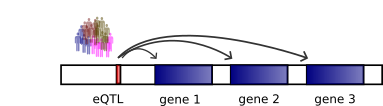
\includegraphics[width=\textwidth]{fig/model1.png}
%    \end{subfigure}
%
%\end{figure}

%  CONFIGURE NEWcitep SINGLE-PAGE FORMAT

\onecolumn % go back to one column
%\fancyhead{} % make sure we get no headers
\renewcommand{\floatpagefraction}{0.1}
%\lfoot[\bSupInf]{\dAuthor}
%\rfoot[\dAuthor]{\cSupInf}
\newpage

%\captionsetup*{format=largeformat} % make figure legend slightly larger than in the paper
\setcounter{figure}{0} % reset figure counter for Supp. Figures
\setcounter{equation}{0} % reset equation counter for Supp. Equations
%\setcounter{page}{1} % reset page count
%\makeatletter
%\renewcommand{\thefigure}{S\@arabic\c@figure} % make Figure legend start with Figure S
%\makeatother
%\def\theequation{S\arabic{equation}}
\renewcommand{\figurename}{Supplementary Figure}

%  MAIN TEXT

\newpage
\section*{Supplementary Information}

%%%%%%%%%%%%%%%%%%%%%%%%%%%%%%%%%%%%%%%%%%%%%%%%%%%%%%%%%%%%%%%%%%%%%%%%%%%%%%%%
%
% Supp fig 1: Percent of explained loci
%
%%%%%%%%%%%%%%%%%%%%%%%%%%%%%%%%%%%%%%%%%%%%%%%%%%%%%%%%%%%%%%%%%%%%%%%%%%%%%%%%

%\begin{figure}[!tbp]
%    \centering
%    \includegraphics[width=\textwidth]{\floatRelativePath/cmpt_perc_tophits_eqtl.py/subplots.png}
%
%    \caption{}
%%
%\end{figure}

%%%%%%%%%%%%%%%%%%%%%%%%%%%%%%%%%%%%%%%%%%%%%%%%%%%%%%%%%%%%%%%%%%%%%%%%%%%%%%%%
%
% Fig 2: ucsc screenshots
%
%%%%%%%%%%%%%%%%%%%%%%%%%%%%%%%%%%%%%%%%%%%%%%%%%%%%%%%%%%%%%%%%%%%%%%%%%%%%%%%%

\begin{figure}[!ht]
    \centering

    \begin{subfigure}[]{0.99\textwidth}
        \textbf{a}
        \\
        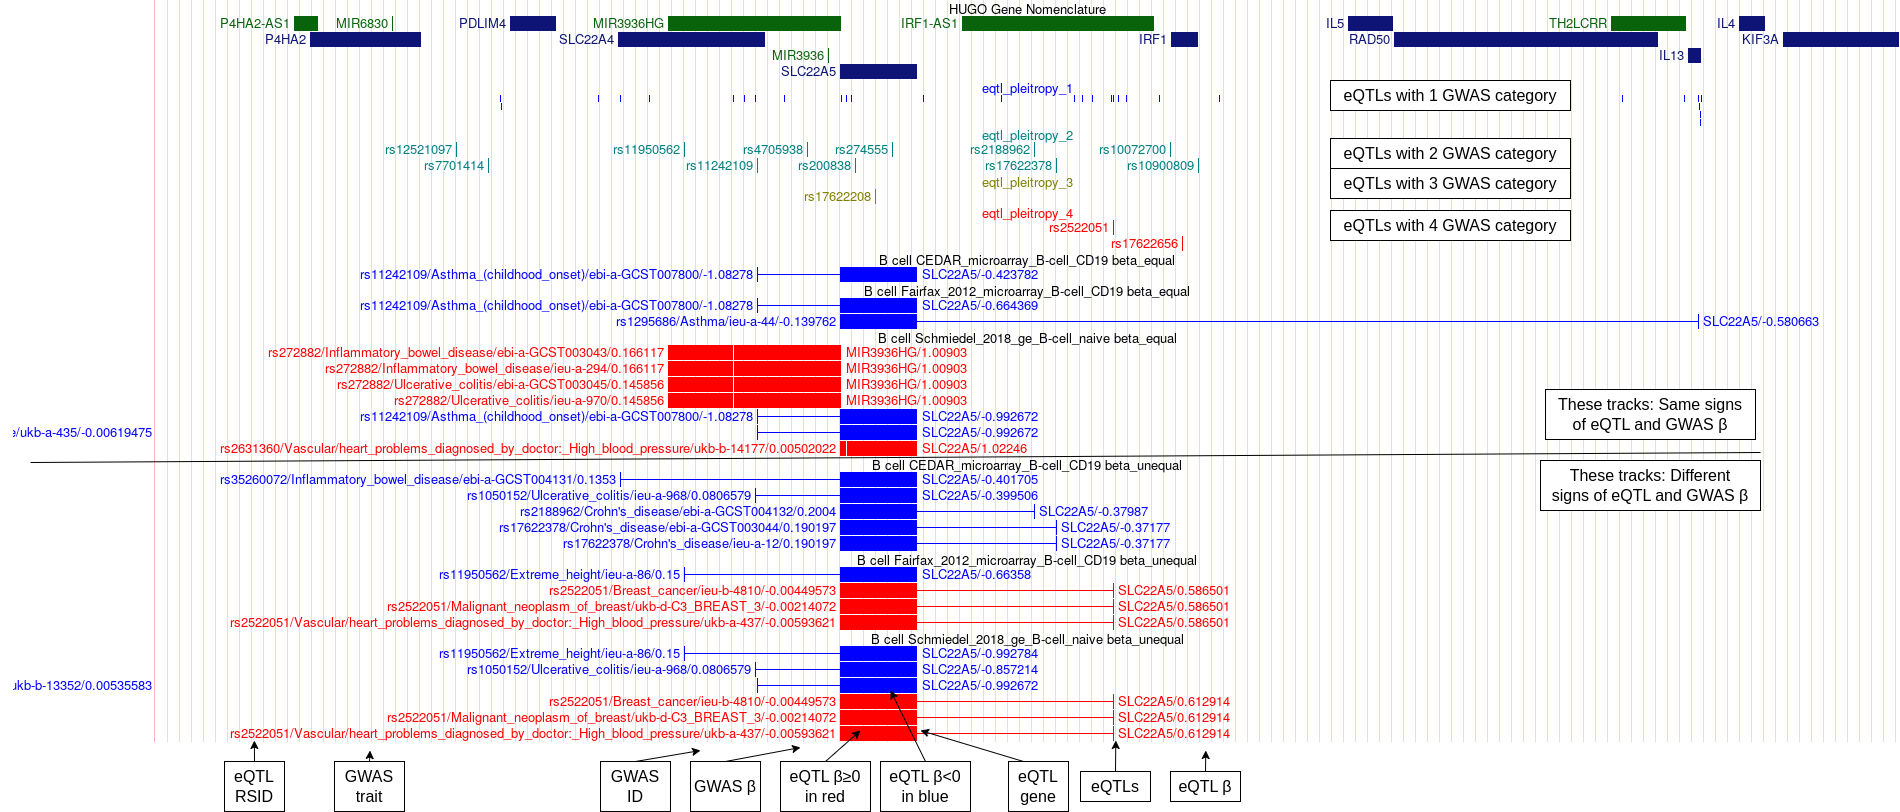
\includegraphics[width=\textwidth]{fig/ucsc_gwas2eqtl_il4_bcell_help.png}
    \end{subfigure}

    \begin{subfigure}[]{0.99\textwidth}
        \textbf{b}
        \\
        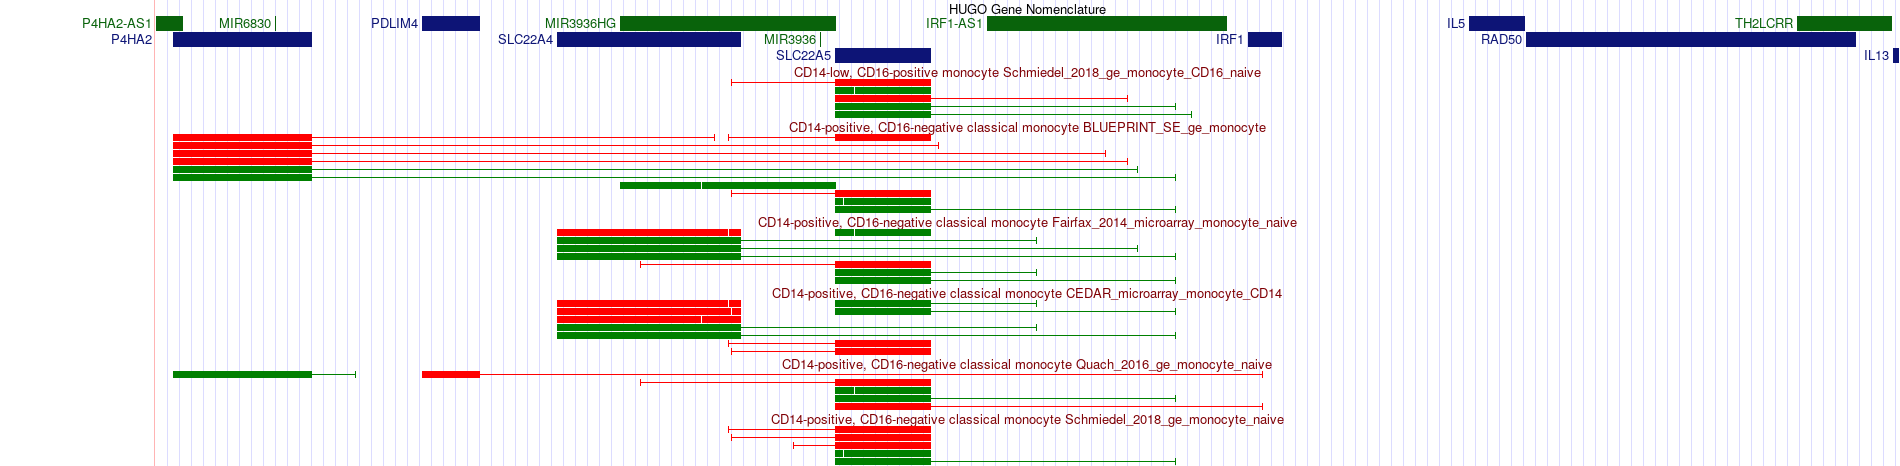
\includegraphics[width=\textwidth]{fig/ucsc_gwas2eqtl_il4_monocyte.png}
    \end{subfigure}

    \begin{subfigure}[]{0.99\textwidth}
        \textbf{c}
        \\
        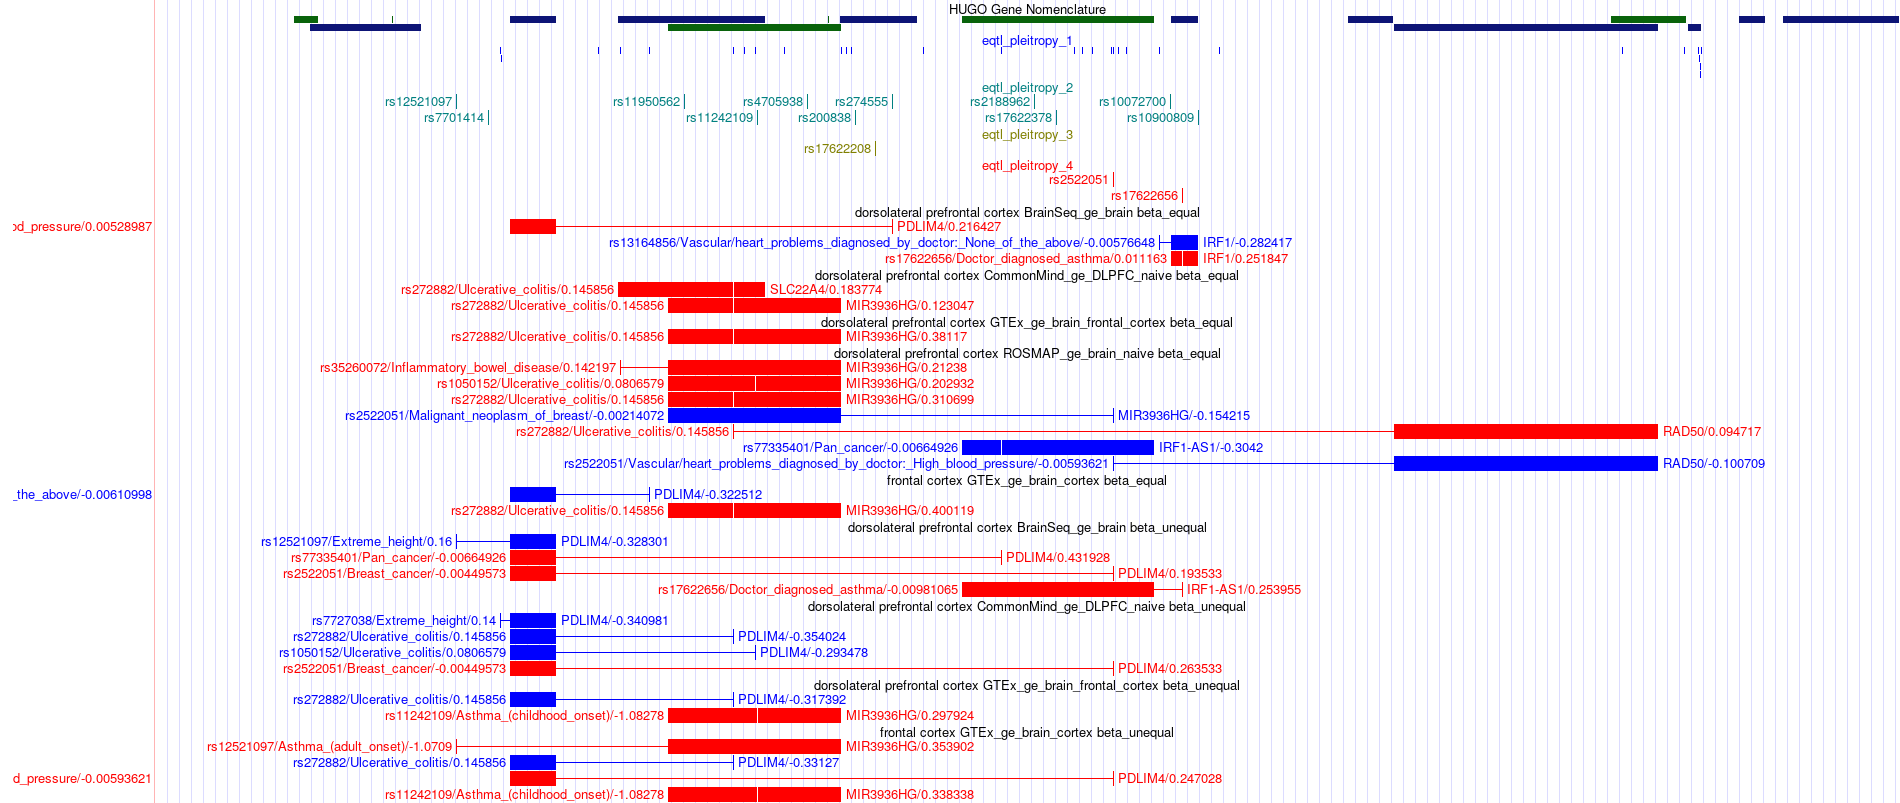
\includegraphics[width=\textwidth]{fig/ucsc_gwas2eqtl_il4_frontalcortex.png}
    \end{subfigure}

    \caption{}

\end{figure}

%%%%%%%%%%%%%%%%%%%%%%%%%%%%%%%%%%%%%%%%%%%%%%%%%%%%%%%%%%%%%%%%%%%%%%%%%%%%%%%%
%
% Fig 5: Comparison with Watanabe 2019
%
%%%%%%%%%%%%%%%%%%%%%%%%%%%%%%%%%%%%%%%%%%%%%%%%%%%%%%%%%%%%%%%%%%%%%%%%%%%%%%%%

\begin{figure}[!ht]
    %
    \centering
    %
    \begin{subfigure}[]{.49\textwidth}
        \textbf{a}
        \\
        \includegraphics[width=\textwidth]{\floatRelativePath/cmpt_count_per_rsid.py/watanabe_cat_count.png}
    \end{subfigure}
    %
    \begin{subfigure}[]{.49\textwidth}
        \textbf{b}
        \\
        \includegraphics[width=\textwidth]{\floatRelativePath/cmpt_count_per_rsid.py/watanabe_percentage.png}
    \end{subfigure}

    \caption{}

\end{figure}

%%%%%%%%%%%%%%%%%%%%%%%%%%%%%%%%%%%%%%%%%%%%%%%%%%%%%%%%%%%%%%%%%%%%%%%%%%%%%%%%
%
% Supp fig: allele frequencies
%
%%%%%%%%%%%%%%%%%%%%%%%%%%%%%%%%%%%%%%%%%%%%%%%%%%%%%%%%%%%%%%%%%%%%%%%%%%%%%%%%

\begin{figure}[!tbp]

    \begin{subfigure}[]{.49\textwidth}
        \textbf{a}
        \\
        \includegraphics[width=\textwidth]{\floatRelativePath/plt_x_per_variant_y_allele_freq.py/amr_af_custom.png}
    \end{subfigure}
%
    \begin{subfigure}[]{.49\textwidth}
        \textbf{b}
        \\
        \includegraphics[width=\textwidth]{\floatRelativePath/plt_x_per_variant_y_allele_freq.py/afr_af_custom.png}
    \end{subfigure}

    \begin{subfigure}[]{.49\textwidth}
        \textbf{c}
        \\
        \includegraphics[width=\textwidth]{\floatRelativePath/plt_x_per_variant_y_allele_freq.py/eas_af_custom.png}
    \end{subfigure}
%
    \centering
    \begin{subfigure}[]{.49\textwidth}
        \textbf{d}
        \\
        \includegraphics[width=\textwidth]{\floatRelativePath/plt_x_per_variant_y_allele_freq.py/eur_af_custom.png}
    \end{subfigure}

    \begin{subfigure}[]{.32\textwidth}
        \textbf{e}
        \\
        \includegraphics[width=\textwidth]{\floatRelativePath/plt_x_per_variant_y_allele_freq.py/sas_af_custom.png}
    \end{subfigure}

    \caption{}

\end{figure}


\begin{figure}[!ht]

    % Fig 9: eQTL gene distance furthest
    \begin{subfigure}[]{.49\textwidth}
        \centering
        \textbf{a}
        \\
        \includegraphics[width=\textwidth]{\floatRelativePath/plt_x_per_variant_y_egene_distance.py/boxenplot_custom_furthest_distance.png}
    \end{subfigure}

    \caption{}

\end{figure}


\begin{figure}[!ht]

    \begin{subfigure}[]{.49\textwidth}
        \textbf{a}
        \\
        \includegraphics[width=\textwidth]{\floatRelativePath/plt_x_per_variant_egene_y_etissue.py/plt.png}
    \end{subfigure}

    \caption{}

\end{figure}





% \bibliographystyle{apalike}
% \bibliography{ms_pleiotropy}
\printbibliography

\end{document}
